%!TEX root= ../../../report.tex

\section{Biomechanics meets Control} % (fold)
\label{sec:biomechanics_vs_control}
The first attempts to accomplish artificial walking machines in the mid-1950s were based on stiff structures and kinematic control.
There has been more than 60 years of development in several technology fields between them and the current soft, compliant and torque-controlled legged robots.
Among the main advances that gave rise to the evolution of the autonomous walking robots, three considered essential and of great relevance for this thesis are listened in \ref{list:leg_advances} and further discussed here.
Thanks to them, nowadays the research in legged robotics goes hand in hand with the study of biological locomotion systems in the attempt to imitate existing features present in nature.

\begin{itemize}
\label{list:leg_advances}
	\item The realization of the importance that a dynamic and active control has on the walking behavior, as opposed to rigid, kinematics-based motion.
	\item The conception of the embodied AI. The influence of the body in the process of thinking.
	\item The improvements in sensors/actuators performance, material science, embedded computing power and power sources.
\end{itemize}

\subsection{The relevance of body dynamics} % (fold)
\label{sub:dynamics_control}
Stiff position control for kinematic trajectory planning has lately demonstrated impressive capabilities for instance during the last DARPA learning locomotion challenge.
However, the limitations of this kind of control such as the need of a very detailed knowledge  about both the robot state vector and the environment have been also exposed.
Thus, it seems clear that the solution for robust and adaptive motion platforms has to go through the development of dynamics-based control models.
The first big steps in dynamic legged locomotion control took place in the 90's in the Leg Laboratory, at the MIT Artificial Intelligence Laboratory carried out by Marc Raibert and his team.
Their findings about the importance of active balance for stability and the possibility of creating simple and generalizable control algorithms for complex dynamic legged systems \cite{mit_leg_lab1} pushed the development of walking robots to a new stage.
Besides, they were among the pioneers in the realization of the influence of the mechanical design together with the control in the generation of complex behaviors in locomotion.
A paradigmatic example of the importance of the biomechanics and the body dynamics in the control of machines intended for locomotion is the well-known passive walker developed by McGeer \cite{passive_walking} and shown in \ref{fig:passive_walker}. 
The achievement of a human-like, efficient walking behavior without any kind control structure gave birth to the concept of morphological computation.

% subsection dynamics_control (end)
\begin{figure}[htb]
	\centering
	\begin{subfigure}[t]{0.35\textwidth}
        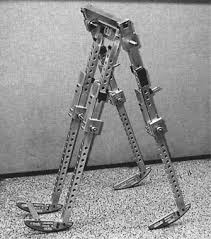
\includegraphics[width=\textwidth]{figures/passive_walker.jpg}
        \caption{McGeer's passive walker.}
        \label{fig:passive_walker}
    \end{subfigure}
    \begin{subfigure}[t]{0.35\textwidth}
        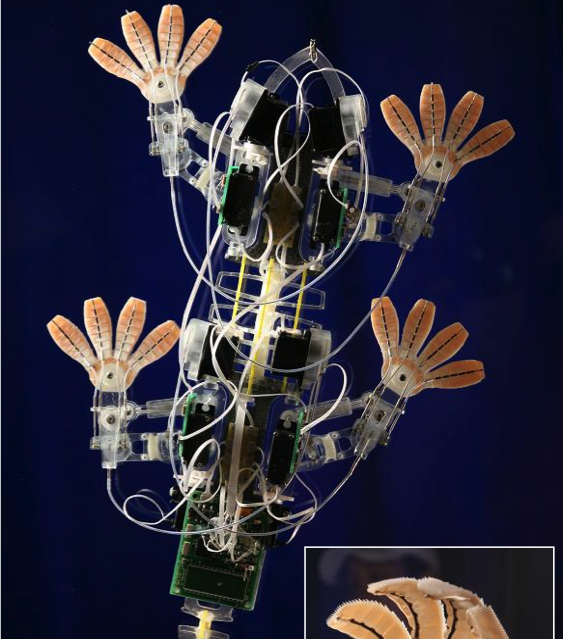
\includegraphics[width=\textwidth]{figures/Stickybot.jpg}
        \caption{Stickybot robot, Standford University.}
        \label{fig:stickybot}
    \end{subfigure}
\caption{Examples of bio inspired mechanics in locomotion.}
\label{fig:figure1}
\end{figure}

\subsection{Embodied AI and locomotion} % (fold)
\label{sub:the_embodiment_}
The embodiment concept came up in the Artificial Intelligence field in the 1980's as a mean to explore the influence of the body and its characteristics in the process of thinking. 
Its aim could be expressed as the search for the answer to the question, in the very convenient words of Rolf Pfeifer and Fumiya Iida, "How does walking relate to thinking?".
As introduced in \cite{pfeifer}, the original goal of AI the understanding of natural forms of intelligence that have more to do with the interaction with the real world rather than the only development of computer algorithms.

The advent of this new approach in AI caused by itself an enormous boost in the field of locomotion in robotics since it made researchers start working with mobile robots.
"The general initial conviction that locomotion and orientation were the underlying driving forces in the development of cognition, in the evolution of the brain, led to the general use of the already available wheeled robots" \cite{pfeifer}.
In the seek of an answer to the famous question "Why don’t plants have brains?", by D. Wolpert, the belief that the reason could be their incapacity for displacement led to an increasing use of mobile robots as a research tool.

Besides, the embodied AI brought about the turn to nature for inspiration in biological systems under the belief that the results of Darwinian evolution and the principle of ecological balance had created systems of greater complexity and efficiency worth studying and mimicking.
With all this, it came the understanding that complex behavior could arise from the synergistic combination of simple algorithms and the physical characteristics of the body.
Since then, mechanical compliance in the actuation, soft materials and bio inspired controllers such as CPGs for instance have been widely studied and implemented in walking machines. 
An example of this concept is the Stickybot, created in the Biomimetics and Dexterous Manipulation Lab at Standford University and shown in Figure \ref{fig:stickybot}.
% subsection the_embodiment_ (end)

\subsection{The advancement of hardware} % (fold)
\label{sub:the_advances_in_hardware}
The early timeline of the evolution in the technology utilized in biped robotic systems can be analyzed taking a look at the progression of the humanoid robots at Waseda University in Japan, in the Humanoid Research Laboratory.
In the late 1960's, Ichiro Kato and his team created the WAP-1, the first version of their first generation of humanoid robots, and the WAM-1 \ref{fig:waseda_robot1}, matching the launching of the first microprocessors.
The WAP-1 robot was moved by very slow pneumatic artificial muscles, first developed in the 1950's but not widely commercialized until the beginning of the 80's, and had to be connected to a large external computer frame for its control. 
Later version WAP-2 and WAP-3 incorporated controller-based memory and PWM-driven actuators, created at the end of the 1960's, that allowed to reach three-dimensional walking at near human-like locomotion speeds for the first time in history.
Kato also created the first full-size humanoid robot, the Wabot-I, and since the beginning of the 80's his group and him applied for the first time 16-bit microcomputers (introduced in 1973) to the implementation of quasy-dynamic walking control \cite{biped_robots_history}.
On of the latest achievements of Kato Laboratory is the WABIAN-2R, in \ref{fig:waseda_robot2}.

\begin{figure}[htb]
	\centering
    \begin{subfigure}[t]{0.3\textwidth}
        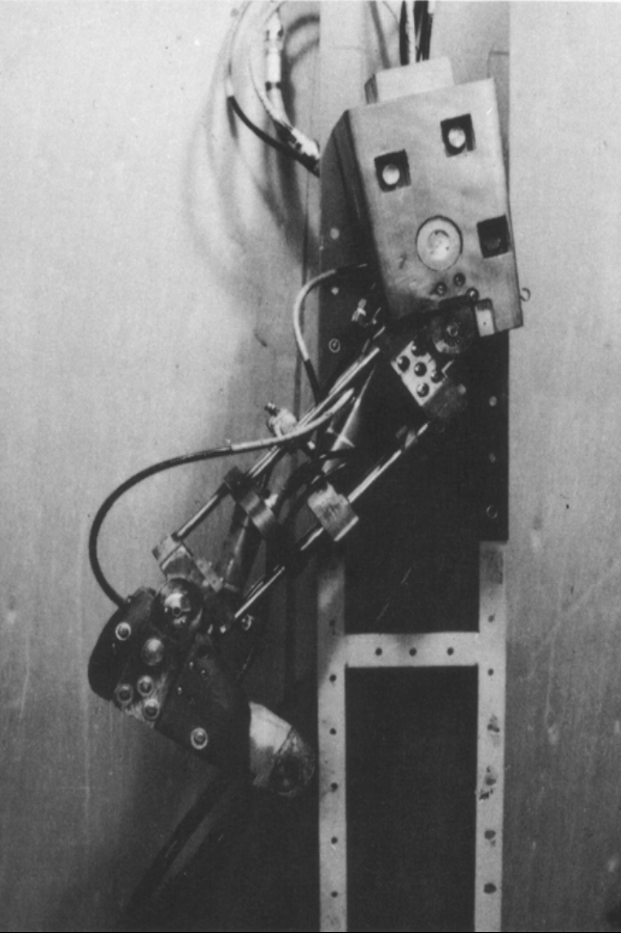
\includegraphics[width=\textwidth]{figures/waseda1.pdf}
        \caption{WAM-1 (1966)}
        \label{fig:waseda_robot1}
    \end{subfigure}
    \centering
    \begin{subfigure}[t]{0.3\textwidth}
        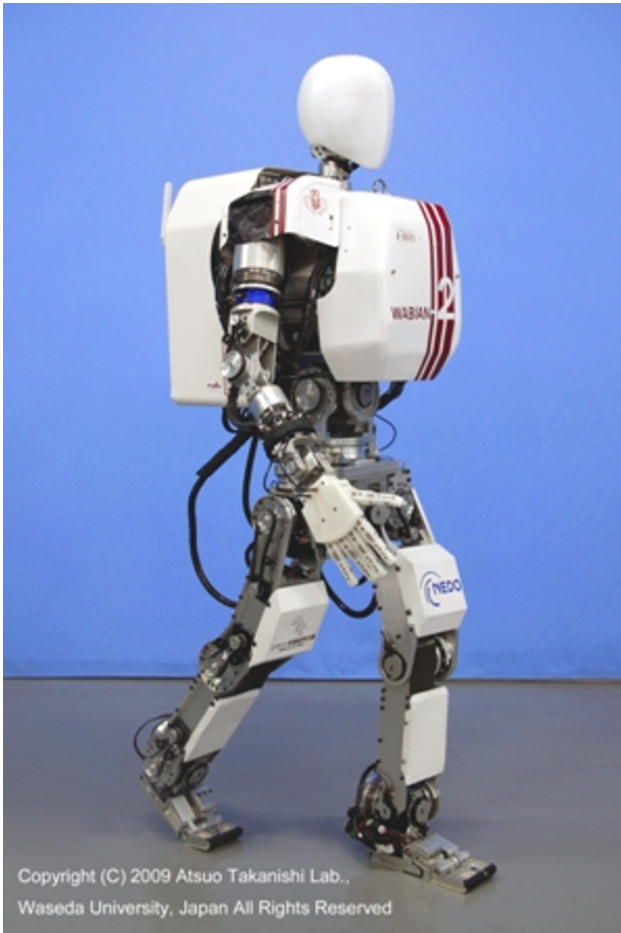
\includegraphics[width=\textwidth]{figures/waseda2.pdf}
        \caption{WABIAN-2R (2006)}
        \label{fig:waseda_robot2}
    \end{subfigure}
    \caption{Examples of humanoid robots.}
\end{figure}

The above is just an example of how during the last two decades of the 20th century and the beginning of the 21st, the progresses in sensing, actuation and control has largely influenced the development of legged locomotion in robotics.
However, despite the latest and impressive enhancements in mechatronics, its evolution continues presenting challenges for the advancement of autonomous biped robots.
Nowadays, the main requirements from a hardware point of view are listed in \ref{list:hardware_challenges} as per \cite{biped_robots_history}.

\begin{itemize}
	\item Energy-efficient and high-performance actuators with high torque-to-weight ratio and high torque-to-volume ratio.
	\item Highly reliable while economical sensors.
	\item Lightweight but mechanically strong materials for construction of the structure and mechanism.
	\item Fast, high computing power, and economical dedicated computer system robust against hostile situations of nature.
	\item Lighter power sources with greater autonomy.
\label{list:hardware_challenges}
\end{itemize}

In spite of this, it seems that the progress in legged autonomous systems will come from the hand of the introduction in the robotics field of recent areas in science as nanotechnology or smart materials.
Together with this, the new findings in microelectronics and the miniaturization of computers and batteries will help overcome the current challenges.


% subsection the_advances_in_hardware (end)


% section biomechanics_vs_control (end)